\documentclass{myreport}
% =============================================
% Part 1 Edit the info
% =============================================

%图片路径,按需要添加,注意末尾要加‘/’
\graphicspath{
{figures/}
{logo/}
}


%封面的课程信息
\renewcommand{\major}{电力电子与电力拖动}
\renewcommand{\institute}{电气工程学院}
\renewcommand{\name}{GQY}
\renewcommand{\stuid}{2171xxxx}
\renewcommand{\newdate}{2018-08-31}
\renewcommand{\courseworktitle}{GQY的一个课程作业标题要长长长长长长长长长来测试换行}
\renewcommand{\coursetitle}{\LaTeX 学习}
\renewcommand{\tutor}{某老师}
\renewcommand{\email}{1234567@email.com}

\begin{document}

%%%%%%%%%%%%%%%%%%%%%%%% 封面 %%%%%%%%%%%%%%%%%%%%%%
\thispagestyle{empty}
\makemycover %封面\makemytitle在.cls里

%%%%%%%%%%%%%%%%%%%%%%%% 封面 %%%%%%%%%%%%%%%%%%%%%%


%\listoffigures 
%%%%%%%%%%%%%%%%%%%%%%%% 正文开始 %%%%%%%%%%%%%%%%%%%%%%

%begin a new page
\clearpage
\newpage

\section{简介}
这是我的课程作业   模板,    准备以后研究生的时候写平时作业或者实验室的报告用,之前没用过中文的Tex,也没自己设计过格式,所以自己练习下\LaTeX。--GQY, 1st Sep 2018. a

使用XeLaTeX和 Tex Live。继续测试github。

顺便发现在中文TeX里似乎两个汉字之间   加空格是无效的,在英文 Tex 里面多个空格看作一个。


\section{章节测试}
section 一、,subsection 1.1,subsubsection (1)。
\subsection{测试subsection2-1}
看下段落的缩进。看下段落的缩进。看下段落的缩进。看下段落的缩进。看下段落的缩进。看下段落的缩进。看下段落的缩进。看下段落的缩进。看下段落的缩进。看下段落的缩进。看下段落的缩进。
\subsubsection{测试subsubsection}
equation测试,\eqref{eq:foo1}是第一个公式
{\color{red}(ref前后需要加空格吗?)}发现\LaTeX 打字中英切换还是麻烦,估计shift键要坏掉了。
\begin{equation}
\int_a^b f(x)dx = 0 \label{eq:foo1}
\end{equation}

align测试,\eqref{eq:align1} 和 \eqref{eq:align2} 是align中的两个公式。测试ref:\ref{eq:align1},测试eqref:\eqref{eq:align1},测试autoref:\autoref{eq:align1}.
\begin{align}
 \bm{a}_b &= a_b \label{eq:align1}\\
 v_{primary} &= L_{\mu 1}\frac{di_{\mu 1}}{dt} \label{eq:align2} 
\end{align}


\subsection{章节测试2-2}
\subsubsection{subsub1}
\subsubsection{subsub2}

\section{图表}
\subsection{图片}
复制了TeX狮的一组图片。
我想在这里放一张图,那就是\autoref{fig:waveform},顺便测试自动引用autoref,修改了figureautorefname。
\begin{figure}[htbp]
\centering

\includegraphics[width=4in]{Chapter1}
\caption{第一张图。}
\label{fig:waveform}
\end{figure}

用subcaption包放一组图,\autoref{fig:subfig_test1}包含了\autoref{subfig:1a}, \autoref{subfig:1b},\autoref{subfig:1c}和\autoref{subfig:1d},复制自浙大研究生论文TeX模板。果然autoref没有错误了,以前用subfig包的时候不会显示“2a”,而只显示“a”。使用换行“\textbackslash\textbackslash” 可以决定每行放多少幅小图,如不换行,默认按照图片大小塞满整行。

\begin{figure}[htbp]
	\centering
	\begin{subfigure}[b]{.4\textwidth}
		\centering
		
\includegraphics[width = \textwidth]{Chapter2}
		\bisubcaption{书籍排版与普通排版}{bicaption in subcaption}\label{subfig:1a} 
	\end{subfigure}
	\quad \\
	\begin{subfigure}[b]{.2\textwidth}
		\centering
		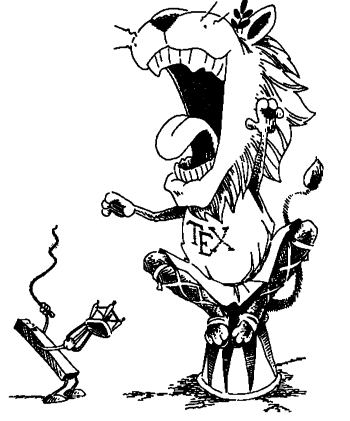
\includegraphics[width = \textwidth]{Chapter3}
		\caption{\TeX 的控制系列}\label{subfig:1b}
	\end{subfigure}
	\begin{subfigure}[b]{.2\textwidth}
		\centering
		
\includegraphics[width = \textwidth]{Chapter4}
		\caption{\TeX 的控制系列}\label{subfig:1c}
	\end{subfigure}
	\begin{subfigure}[b]{.2\textwidth}
		\centering
		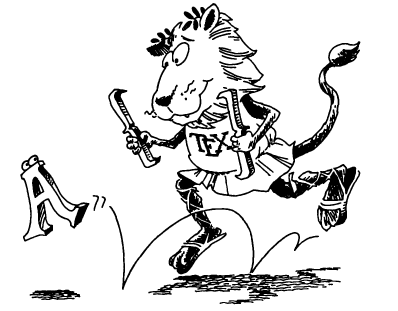
\includegraphics[width = \textwidth]{Chapter5}
		\caption{\TeX 的控制系列}\label{subfig:1d}
	\end{subfigure}
	\bicaption{子图模式测试1:2张图}{bicaption in subfigure
	}\label{fig:subfig_test1}
\end{figure}

\subsection{表格}
我从隔壁拿过来一张表格,\autoref{tb:test1}。

\begin{table}[!h]
\caption{一张表格}
\label{tb:test1}
\centering
\begin{tabular}{ll}
\hline
名称              & 值              \\ \hline
表格测试二        & 6 mH               \\
表格测试三         & $\mathrm{5\: m\Omega}$ \\
表格测试四 & 50 Hz               \\ 
表格测试五 & 3 kHz \\ 
表格测试六      & $\mathrm{\frac{1}{3000}\;s}$     \\ \hline
\end{tabular}
\end{table}

插入一段matlab代码。
\lstinputlisting[language=MATLAB]{code/sample.m}
%插入一段长一点的matlab代码
%\lstinputlisting[language=MATLAB]{code/pr_bode.m}



\end{document}
